This section will deal with theoretical components from our project. Here, linear circuit analysis gives noise and output voltage relationship. 

\subsection{Linear circuit analysis \label{lca}}


We have a voltage regulator circuit from a zener diode which regulates voltages at specific voltage known as zener voltage $V_{z}$. The fluctuation from these regulated voltages is what we call noise. Since ideal regulators only give pure DC voltages at output, this fluctuation is completely unwanted and only be resultant of intrinsic noise of this regulator circuit.  We limit ourselves with only noise coming from zener diode which is not quite good practice. Since, noise can be added from extra resistors, wires and even the power supply itself. The resistor noise can be neglected because of their low values as we used 10k in series and 100k in parallel to output. We will see this later.

Let’s take a basic voltage regulator circuit as shown in figure \ref{thcir1}.

\begin{figure}[hbt!]
\centering{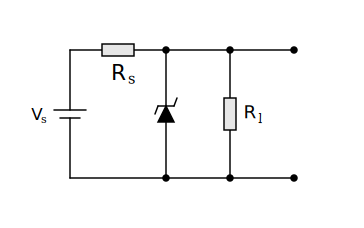
\includegraphics[width=.48\textwidth]{circuit-20231005-2243.png}}
\caption{Simple voltage regulator circuit made from zener diode \label{thcir1}}
\end{figure}

As you can see we have a zener diode parallel to the power supply, which regulates at a certain degree. Since this is a linear circuit output voltage can be easily derived.

Applying kirchhoff current low in the figure \ref{thcir1},


\begin{align*}
I_{z} & = I_{R_s} -I_{L}\\
& = \frac{V_s-V_o}{R_s}-\frac{V_o}{R_L}\\
& = -V_o(\frac{1}{R_s}+\frac{1}{R_L})+ \frac{V_s}{R_s}\\
& = -V_oA^{\prime}+B^{\prime}
\end{align*}

Here, $A^{\prime} = (\frac{1}{R_s}+\frac{1}{R_L})$ and $B^{\prime} = \frac{V_s}{R_s}$.  

We can write $I_z = \frac{V_z}{R_z}$, where $V_z$ and $R_z$ are respectively zener voltages and impedance.  This relation is quite linear in the breakdown region as you can see in the figure \ref{thiv}. \footnote{Image is taken from Electronics Devices and Circuit Theory by Robert Boylsted}

\begin{figure}[hbt!]
\centering{\includegraphics[width=.48\textwidth, trim={.8cm 0.6cm .8cm .5cm},clip]{thzenerIV.png}}
\caption{theoretical current and voltage relation for zener diode \label{thiv}}
\end{figure}


Here we can assume equivalent circuit of \ref{thcir1} as figure \ref{thcir2} 

\begin{figure}[hbt!]
\centering{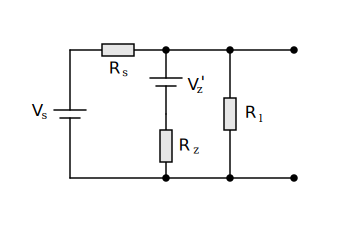
\includegraphics[width=.48\textwidth]{circuit-20231005-2244.png}}
\caption{Equivalent circuit of figure \ref{thcir1} \label{thcir2}}
\end{figure}

Further, simplifying the circuit,

\begin{figure}[hbt!]
\centering{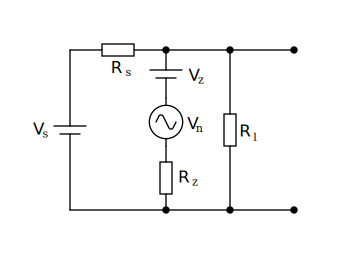
\includegraphics[width=.48\textwidth]{circuit-20231005-2245.png}}
\caption{Equivalent circuit of figure \ref{thcir2} \label{thcir3}}
\end{figure}

This circuit is further simplified as we take $V_z = V_{DC} + V_n$ where $V_n$ is the noise voltage of the zener diode.
If we neglect noise from other sources like resistors and power supply then from figure \ref{thcir3},

\begin{align*}
\frac{V_z}{I_z} & = -V_oA^{\prime} +B^{\prime}\\
\frac{V_{DC}+V_n}{I_z} & =  -V_oA^{\prime} +B^{\prime}\\
V_n & = -V_oA+B
\end{align*}


\begin{align} \label{vo}
V_o & = -\frac{V_n}{A}+\frac{B}{A}
\end{align}



So, we can conclude that here as $V_o \propo V_n$.  This will be the main focus of this project. Here we are neglecting $V_{DC}$ and will be totally okay when we read data from the LOCK IN amplifier, since the DC component has zero frequency which can’t be read from the LOCK IN amplifier.

\subsection{Different noises in the circuit \label{thno}}

The noise voltage $V_n$ is made from different types of noise source which can act as a symbol voltage source. So, $V_n$ can be broken into sub noise sources such as $V_n = V_{flicker}+V_{thermal} + V_{shot} +\cdots$. We will see this noise source and its origin then we will derive its respective distribution and equations.\cite{reggiani1997monte}\cite{wilamowski2018fundamentals}

\begin{figure}[hbt!]
\centering{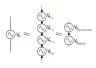
\includegraphics[width=.48\textwidth]{noiseeq.png}}
\caption{Equivalent noise sources}
\end{figure}

\subsubsection{Flicker Noise \label{thflicker}}

Flicker noise is also known as 1/f noise in view of the fact that power density decreases with increasing frequency. This implies that at lower frequencies, the flicker noise dominates.
This type of noise is found  almost in any electronic device which is able to operate at lower frequencies.The main source of this type of noise is D.C supply. Its first evidence was given by J. B. Johnson \cite{johnson1925schottky}. Its first 1/f form is derived by beck and spruit \cite{beck19781}. Now the form is given as 

\begin{align}
S(f) & = \frac{\gamma}{f^{\alpha}}
\end{align}

Here, $\gamma$ and $\alpha$ determine the nature of flicker noise. $\alpha$ determine relations with other noise elements.

\begin{enumerate}
\item ($\alpha > 0$): This means that white noise is dominating the flicker noise as frequency increases.
\item ($\alpha = 0$): This means that only white noise is exists
\item ($\alpha < 0$): This means noise is increasing as frequency. Also, shows that noise will be persistent with a higher range of frequencies. Typically white noise dominates traditional flicker noise.
\end{enumerate}

We can see noise levels as from figure \ref{thnoise}. mostly flicker noise is at considered as $1/f$ noise. In which $\alpha = 1$.

\subsubsection{$1/f^2$ noise}
$1/f^2$ noise is a derivative of  $1/f$ noise and it's mostly seen in metal interconnections of intregrated circuits.

It is modeled by following,
\begin{align*}
  S_{1/f^2}(f) = C \frac{j^{\beta}}{f^{\gamma}\cdot T}\cdot e^{\frac{-E_a}{kT}} 
\end{align*}

Here, C is costant which can be found from experiment, $E_a$ is activation energy for electromigration, $k$ is boltzmann contant, $T$ is temperature. $j$ is current density, $\beta$ and $\gamma$ are contants canbe found from experiment. ($\beta \geq 3$ and $\gamma \geq 2$).
\subsubsection{Shot noise \label{thshot}}

Shot noise is a form of noise that arises because of the discrete nature of the charges carried by charge carriers, electrons or holes or photons hitting the surface. Shot noise is analogous to the rainfall in which raindrop hitting the surface can be considered as discrete. The sound of rainfall is very similar to noise we hear from speakers when we are considering shot noise. Foundational studies in shot noise done my campbell.\cite{campbell1909study}

Since, shot noise is a phenomenon for discrete charge passing through a junction, it can be modelled by poisson distribution. Suppose that In the time interval the $\tau$ Q charge passes through a junction in a semiconductor device (in present context zener diode). This gives rise to discrete probability distribution,

\begin{align}
P(N) & = \frac{e^{-\lambda \tau}(\lambda \tau)^{N}}{N!}
\end{align}

If $N=0$ charge passes in time interval $\tau$ then $P(N)$will be,

\begin{align} \label{eqN0}
P(0) & = e^{-\lambda \tau}
\end{align}

Now suppose, probability of one and only one charge passing through junction in time $\tau$,

\begin{align*}
P(\tau)d\tau & = (P_{\tau}(0))(P_{\tau}(1))
\end{align*}

From equation \ref{thN0},


\begin{align*}
P(\tau)d\tau & = (e^{-I_0 \tau})(e^{-I_0 d\tau} I_0 d\tau)\\
P(\tau) & = (e^{-I_0 (\tau + d\tau)}) I_0
\end{align*}

We can write this equation in frequency domain and by,

\begin{align}\label{thgenl}
P(f) & = S df
\end{align}

Where S is the spectral density of noise.

Here we can write specific form for shot noise in equation \ref{thgen}.\cite{campbell1909study}

%% \cite{campbell}

\begin{align}\label{thshotvo}
\langle V_{shot}^2\rangle & = 2 e I_0 df
\end{align}

Here, $e$ is electron charge,

$I_0$ is average current,

$df$ is ENBW = Equivalent Noise Bandwidth

\begin{align}\label{thshots}
S(f) & = 2 e I_0
\end{align}

\begin{figure}[hbt!]
\label{thnoise}
\centering{\includegraphics[width=.48\textwidth]{thnoise.png}}
\caption{Equivalent noise sources}
\end{figure}

This spectral density gives independence to frequency, which is called white noise. 


\subsubsection{Avalanche or zener noise \label{than}}

avalanche noise often considers the device's operating characteristics in the avalanche breakdown region. It is a major problem where the device is working in avalanche breakdown regions. It is multiplicative noise where chains of electrons crossing from junction rise to noise behaviour. It is very similar to shot noise and we can use that model and just use a multiplicative element in it. In our circuit this is significant since we are dealing with zener diode. With potential gradient inside the zener diode, if any hole and electron pair generates, it gets dragged by potential and hits the other lattice. This creates chain reaction and very high amplitude noise measured.


\begin{align*}
\langle V_{avalanche}^2\rangle & = M \langle V_{shot}^2\rangle
\end{align*}

\begin{align}\label{thavvo}
\langle V_{avalanche}^2\rangle & = 2 e M I_0 df
\end{align}

So, the spectral density $S(f)$ of this noise will be nearly white.
 
Here, we can combine this both avalanche and shot noise to make one noise source,

\begin{align*}
\langle V_{s}^2\rangle & = \langle V_{shot}^2\rangle+\langle V_{avalanche}^2\rangle\\
& = 2 e I_0 df + 2 e M I_0 df\\
& = (M+1) 2 e I_0 df\\
\end{align*}

And spectral density will be $S(f) = (M+1) 2 e I_0$

Since this noise is white noise we can measure at every frequency. This is what we are going to do in the next chapter.



\subsubsection{Thermal noise \label{thth}}

Thermal noise, also called Johnson–Nyquist noise is the electronic noise generated by random motion of charge carriers. This charge carrier is generated by the thermal agitation inside an electrical conductor at equilibrium, which happens regardless of any applied voltage. Because of their random motion it can be said that they have a mean value at zero. This reason says that we can't model this noise by poisson distribution but have to model with normal or gaussian distribution. In 1936, J B Johnson first gave an idea about thermal noise in thermionic valves. \cite{johnson1928thermal}

The noise amplitude is very similar to that of shot noise and given as,

\begin{align}\label{ththvo}
\langle V_{thermal}^2\rangle & = 4 K_B R df
\end{align}

Here, $K_B$ is boltzmann constant,

R is resistance of device or component,

$df$ is ENBW.

\begin{align*}
S(f) & = 4 K_B R
\end{align*}


By equation \ref{thths} we can see that thermal noise in an ideal resistor is approximately white, meaning that the power spectral density is nearly constant throughout the frequency spectrum. But practically it does decay to zero at extremely high frequencies (terahertz for room temperature). Also, we are neglecting quantum effects. 


Total noise in the circuit will bre frequency dependent noise and white noise,


\begin{align*}
V_n & = V_{n}(f)+ V_{white}\\
S(f) & = \frac{\gamma}{f^{\alpha}}+(2e(M+1)I_0+4K_bR)+\mathcal{O}(other)
\end{align*}

\begin{align}\label{theoryvn}
S(f) & \approx \frac{\gamma}{f^{\alpha}}+(2e(M+1)I_0+4K_bR)
\end{align}

which is main derivation of our project.

